\chapter{Технологическая часть}

\section{Средства реализации программы}

В качестве СУБД была выбрана графовая база данных Neo4j~\cite{neo4j}.

Обоснование выбора:
\begin{itemize}
    \item \textbf{Природа данных.} Социальные сети естественным образом моделируются в виде графа: пользователи представляют вершины, а их связи — рёбра. Использование графовой модели позволяет органично отразить структуру предметной области.
    
    \item \textbf{Поддержка иерархических и кластерных структур.} Графовые СУБД, в частности Neo4j, позволяют эффективно представлять и обрабатывать иерархические отношения и структуры сообществ, что критически важно при решении задачи выявления сообществ в графе.
    
    \item \textbf{Язык запросов Cypher.} Neo4j использует декларативный язык Cypher, специально разработанный для удобной и наглядной работы с графами. Это упрощает реализацию сложных запросов к структуре графа и уменьшает объём императивного кода.
    
    \item \textbf{Активное сообщество и документация.} Neo4j имеет широкую пользовательскую базу, активную поддержку и большое количество обучающих материалов, что упрощает разработку и отладку приложений.
\end{itemize}

Таким образом, выбор Neo4j обусловлен структурой данных задачи, необходимостью обработки иерархий и сообществ, а также производственными и удобочитаемыми преимуществами графовой модели по сравнению с реляционными СУБД.

В качестве языка программирования для реализации курсовой работы был
выбран язык C\# по следующим причинам:

\begin{itemize}
\item в стандартной библиотеке языка присутствует поддержка всех
структур данных, выбранных по результатам проектирования;
\item высокая производительность;
\item наличие официального драйвера для взаимодействия с Neo4j;
\item наличие актуальной документации.
\end{itemize}

\section{Визуализация данных}

Для демонстрации данных был выбран стандартный браузер Neo4j. На рисунке~\ref{fig:data} приведён пример визуализации данных.

\begin{figure}[H]
	\centering
	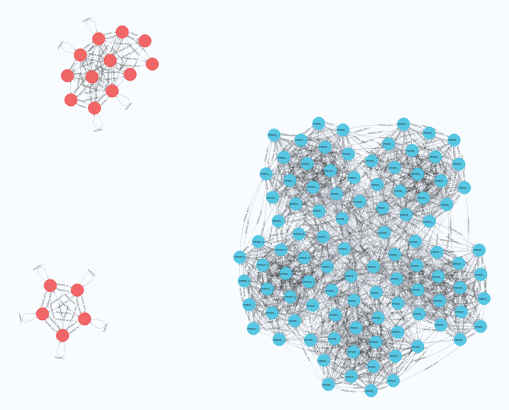
\includegraphics[height=0.4\textheight]{data.png}
	\caption{Пример визуализации данных}
	\label{fig:data}
\end{figure}

\section*{Вывод}

В технологической части был обоснован выбор средств реализации программного обеспечения. В качестве базы данных использована графовая СУБД Neo4j, которая наиболее полно отражает природу предметной области, связанную с моделированием социальных графов и иерархических структур сообществ. Её язык запросов Cypher и встроенная поддержка работы с графами позволили упростить реализацию операций над данными.

Для разработки программной логики выбран язык C\#~\cite{Csharp}, обеспечивающий высокую производительность, удобную работу с асинхронностью и наличие официальной поддержки драйвера для Neo4j. 

Визуализация структуры графа и результатов работы алгоритма осуществляется средствами встроенного браузера Neo4j, что позволило наглядно продемонстрировать полученные данные без необходимости использования сторонних решений.

Выбор указанных технологий обеспечил удобство, надёжность и расширяемость при реализации поставленной задачи.

